\section{Hardware }
This section shows the hardware specifications with which the testing was performed. 

\subsection{Computer}
	The computer used for testing the software is a Mountain f-11 Ivy. Its technical specifications are the following: 

	\begin{figure}[H]
		\begin{center}
	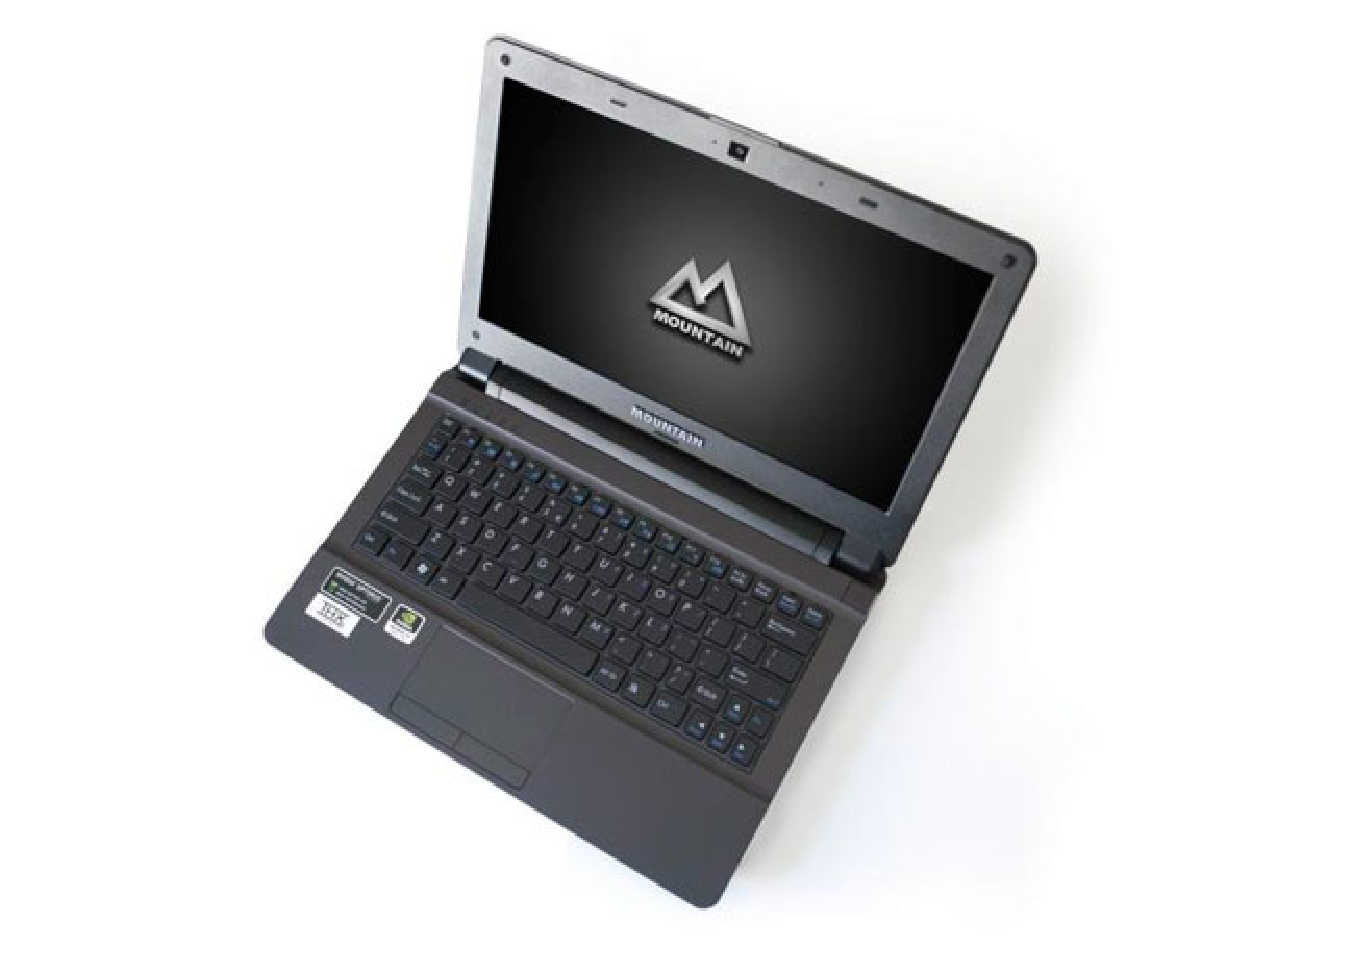
\includegraphics[scale=0.3]{img/mountain.eps}
		\caption[Mountain laptop]{Mountain f-11 Ivy Laptop}
		\end{center}
	\end{figure}

	\paragraph{Processing Units} \mbox{}\\
		\begin{itemize}
			\item{CPU: Intel Core i7-3630QM at 2,40 GHz, Turbo Boost up to 3,4 GHz.}
			\item{Integrated GPU:  Intel HD Graphics 4000 at 650 MHz,  Turbo up to 1.1 GHz }
			\item{Dedicated GPU: NVidia GeForce GT 650M with 2 GB of DR3 memory at 835 MHz }
		\end{itemize}

		\vspace*{0.5cm}

	\paragraph{Memories} \mbox{}\\
		\begin{itemize}
			\item{RAM : 8 GB Kingston HyperX at 1.600 MHz }
			\item{SSD : Kingston HyperX 3K, 120 GB}
		\end{itemize}
		\vspace*{0.5cm}

	\paragraph{Other specifications}
		\begin{itemize}
			\item{Screen: 11.6 '' LED }
			\item{Ports: 3 x USB 3.0 , 1 x USB 2.0 , 1 x HDMI, 1 x VGA, 2 x audio jacks}
			\item{Battery: 6 cells}
			\item{Weight: 1.8kg}
		\end{itemize}
		\vspace*{0.5cm}

	\paragraph{Operating System and Kinect drivers}\mbbox{}\\
		\begin{itemize}
			\item{OS: Ubuntu 13.04, 64 bits}
			\item{Drivers: OpenNI SDK v1.5.4.0, 64bits}
			\item{Drivers: Avin2-v0.93-5.1.2.1}
			\item{Drivers: NITE v1.5.2.21, 64 bits}

		\end{itemize}
		\vspace*{0.5cm}

\subsection{RGB-D sensor}
	The RGB-D sensor used in the testing process is a Kinect 360. Its technical details are the following: 
	\begin{figure}[H]
		\begin{center}
	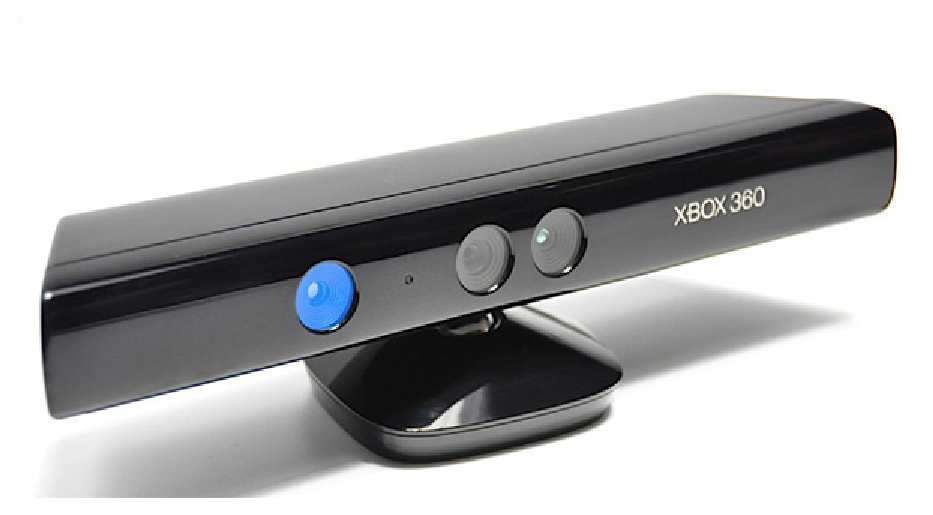
\includegraphics[scale=0.3]{img/kinect.eps}
		\caption[Kinect image]{Kinect for XBOX 360}
		\end{center}
	\end{figure}
	\paragraph{ Sensor} \mbox{} \\
		\begin{itemize}
			\item Colour and depth-sensing lenses
			\item Voice microphone array
			\item Tilt motor for sensor adjustment
			\item Fully compatible with existing Xbox 360 consoles
		\end{itemize}
		\vspace*{0.5cm}

	\paragraph{ Field of View} \mbox{} \\
		\begin{itemize}

			\item Horizontal field of view: 57 degrees
			\item Vertical field of view: 43 degrees
			\item Physical tilt range: ± 27 degrees
			\item Depth sensor range: 1.2m - 3.5m
		\end{itemize}
		\vspace*{0.5cm}

	\paragraph{ Data Streams} \mbox{} \\
		\begin{itemize}

			\item 320x240 16-bit depth @ 30 frames/sec
			\item 640x480 32-bit colour@ 30 frames/sec
			\item 16-bit audio @ 16 kHz
		\end{itemize}
		\vspace*{0.5cm}
